\documentclass[journal]{IEEEtran}

\usepackage{url}
\usepackage{pstricks}
\usepackage{epsfig}
\usepackage{cite}
\usepackage[cmex10]{amsmath}


\begin{document}
\title{Model Order Selection in Reversible Image Watermarking}
\author{Ming~Chen,
        Zhenyong~Chen,
	Xiao~Zeng,
	Zhang~Xiong
\thanks{Manuscript received April 18, 2009; revised October 21, 2009; accepted December 03, 2009.
First published April 26, 2010; current version published May 14, 2010. The associate editor
coordinating the review of this manuscript and approving it for publication was Dr. Michael
Wicks.}%
\thanks{The authors are with the School of Computer Science and Engineering, Beihang University,
Beijing, 100191, China (e-mail: mingchen@cse.buaa.edu.cn; chzhyong@buaa.edu.cn;
zengxiao29@cse.buaa.edu.cn; xiongz@buaa.edu.cn).}%
\thanks{Digital Object Identifier 10.1109/JSTSP.2010.2049222}}


% The paper headers
\markboth{IEEE JOURNAL OF SELECTED TOPICS IN SIGNAL PROCESSING, VOL. 4, NO. 3, JUNE 2010}%
{Ming Chen \MakeLowercase{\textit{et al.}}: Model Order Selection in Reversible Image Watermarking}

\maketitle

\begin{abstract}

Digital watermarking is becoming increasingly important in a large number of applications such as
copyright protection, content authentication and document annotation. Thanks to its capability of
exactly recovering the original host, reversible image watermarking, a kind of digital watermarking,
is favored in fields sensitive to image quality like military and medical imaging. This paper
presents theoretical examination and experimental analysis of model order selection in reversible
image watermarking. It involves two modeling tools: prediction and context modeling. Classic
prediction models are compared and evaluated using specially derived criteria for reversible image
watermarking. Among them, the CALIC, a tool combining the Gradient-Adjusted Prediction with a
context modeling, stands out as the best by providing the most competitive model-fitness with
relatively low complexity. In addition, full context prediction, a model unique to reversible image
watermarking is also discussed. By exploiting redundancy to greater extent, it achieves highly
fitted modeling at a very low order. Experimental results demonstrate that it is capable of
providing even better performance than the CALIC with only negligible computation. 

\end{abstract}

\begin{IEEEkeywords}
Full context prediction, model order selection, prediction-error expansion, reversible image watermarking
\end{IEEEkeywords}

\IEEEpeerreviewmaketitle

\section{Introduction}

\IEEEPARstart{D}{igital} media is rapidly changing the way people work and entertain. Along with
the digital infrastructure of digital signal recorders, processors, communicators, players and
broadcasters, many digital media related applications and techniques are emerging and evolving.
Digital watermarking is such a promising technique. In Wikipedia, digital watermarking is ``the
process of possibly irreversibly embedding information into a digital signal''. In Cox's book
\cite{Cox06book}, watermarking is defined as ``the practice of imperceptibly altering a work to
embed a message about that work''. Both definitions highlight its main character of information
embedding. Digital watermarking is mostly used in copyright protection. It can work either in an
active way to allege ownership of intellectual property, or in a passive way to identify and
prosecute copyright violators. When applied to content authentication, fragile watermarks vulnerable
to malicious manipulation are embedded into digital documents before transmission on unsafe
channels. Once the digital copies are transmitted, their integrity and authenticity can be verified
by detecting those fragile watermarks \cite{Fridrich02invertibleauth}. Digital watermarking is also
capable of managing and annotating digital documents by embedding descriptive information. A well
known case is the watermarking of videos taken by Unmanned Aerial Vehicle (UAV) of the US
army\cite{Marcinak05}. Other applications of digital watermarking include broadcast monitoring,
transaction tracking, access control, legacy enhancement and even more\cite{Cox06book}.  

Although hosts are altered imperceptibly, digital watermarking still introduces permanent distortion
due to replacement, quantization, round-off or truncation \cite{Fridrich02lossless}. This distortion
is intolerable when exact representation of the original host is demanded, e.g. the watermarking for
valuable documents such as military images. In these scenarios, reversible watermarking, which can
recover the original host through watermark extracting, is desired and required. Since the first
invention of reversible watermarking in 1997 \cite{Barton97Patent}, many reversible watermarking
schemes have been proposed. In quite recent years, a set of schemes using prediction-error
expansion \cite{Thodi07,Kuribayashi08,Chang08pe,Chen09add,Chen09full,Tsai09pe,Weng09pe,Hu2009} were
reported to provide outstanding performance in both embedding capacity and image fidelity. These
schemes accomplish reversible watermark embedding by expanding the differences between original and
predicted values of pixels, i.e., prediction-errors. Prediction-error expansion is a generalization
of difference expansion (DE) \cite{Tian03de} by applying expansion to prediction-errors instead of
inter-pixel differences. Since prediction-errors have been proved to be of excellent decorrelating
abilities, they are superior to inter-pixel differences in expandability.

In reversible image watermarking using prediction-error expansion, the calculation of
prediction-errors is a significant and computation-consuming part of the whole process. It involves
a prediction stage and an optional context modeling stage. Prediction decorrelates pixels by
exploiting low order redundancy within local areas, whereas context modeling achieves further
decorrelation by exploiting high order structures, such as texture patterns, via a feedback
mechanism. For both modeling tools, a proper model order is important. Model order affects the
system performance and the implementation complexity in opposite directions. To balance these two
effects, many model order selection criteria have been proposed. A well known criterion is the
Akaike Information Criterion (AIC) named after Akaike \cite{Akaike1974}, which selects a model that
minimizes the expected error using maximum likelihood estimation (MLE). The other one is the Minimum
Description Length (MDL) introduced by Rissanen \cite{Rissanen1984}, which takes the simplest model
sufficiently describes the data to be the best. Both the AIC and the MDL criteria achieve efficient
tradeoff by incorporating terms that penalize the selected model order as it goes high. There also
exist some derivatives of AIC and MDL, and other criteria based on different theories. Though the
model order selection criteria such as AIC and MDL are theoretically well established, they are not
directly applicable in practical scenarios. In real applications, the penalty associated with model
order should be related to the overall system performances and the implementation complexity, which
are not well embodied in these criteria. To provide guidance in the specific application background
of reversible image watermarking, we need special studies regarding this topic.

In this paper, we study the model order selection in reversible image watermarking via theoretical
examination and experimental analysis. To achieve an efficient tradeoff for reversible image
watermarking, specific measures of the model-fitness and the implementation complexity in reversible
image watermarking are derived. Then a set of models, in both prediction and context modeling with
orders varying from low to high, are studied and compared in the derived measures. They include many
well-known predictors including the JPEG predictors, the MED predictor \cite{Loco00ip}, the GAP
predictor \cite{Wu97calic2}, the least-square predictor \cite{Wu98icip, Li01edp, Kau05lsap}, and the
CALIC context modeling scheme \cite{Wu97calic2, Wu97calic}. Although these models are borrowed from
predictive image compression, our study will show very different results which are explainable
because of the distinctive model-fitness criteria in reversible image watermarking. Unlike the case
in predictive image compression, the prediction context in reversible image watermarking is no
longer restricted to half enclosing causal pixels. Without this limit, we can model the prediction
in a more efficient manner and achieve higher model-fitness with even lower model order.

The rest of this paper is organized as follows. Reversible image watermarking using prediction-error
expansion is introduced in Section \ref{sec:watermark}. Measures for the model-fitness and the
implementation complexity are derived in Section \ref{sec:indicator}. Then the model order
selection issue in prediction and context modeling are discussed respectively in Section
\ref{sec:low} and Section \ref{sec:high}. Full context prediction, the modeling technique unique to
reversible image watermarking, is studied in Section \ref{sec:full}. Experimental results of
concrete reversible watermarking schemes employing studied techniques are presented and evaluated in
Section \ref{sec:result}. Finally, conclusions are drawn in Section \ref{sec:conclution}.

\section{Reversible Image Watermarking Using Prediction-Error Expansion}\label{sec:watermark}

A reversible watermarking system, depicted in Fig.\ \ref{fig:wmsys}, consists of two main
procedures, i.e., embedding and extracting. Essentially, reversible watermarking exploits redundancy
in host to provide extra payload for watermark. So it is desired that the host image is transformed
into a domain where pixels are well decorrelated. Prediction-error is such a domain, which is
verifiable in those latest reversible image watermarking schemes
\cite{Thodi07pee,Kuribayashi08,Chang08pe,Chen09add,Chen09full,Tsai09pe,Weng09pe,Hu2009}. As to the
data embedding strategy, difference expansion (DE) \cite{Tian03de} is an outstanding one in both
embedding capacity and image quality. Applying DE to prediction-error, we identify a set of schemes
with excellent performance, i.e., reversible image watermarking using prediction-error expansion. 

\begin{figure}[t]
    \centering
    \includegraphics[width=7cm]{artwork/system.mps}
    \caption{\label{fig:wmsys}A reversible watermarking system. ``Embed'' combines the host
    $\mathbf{x}$ with watermark data $\mathbf{w}$ to form a composite signal $\mathbf{x'}$ under the
    control of a encryption key $\mathbf{k_{em}}$. Importantly, $\mathbf{x'}$ is necessarily close
    to $\mathbf{x}$ in perception. ``Extract'' separates the watermark data $\mathbf{w}$ from the
    composite signal $\mathbf{x'}$ and recover the original host $\mathbf{x}$ with a decryption key
    $\mathbf{k_{ex}}$. The transmission of $\mathbf{x'}$ is considered to be noise-free in this
    paper. }\medskip
\end{figure}

\subsection{Prediction-Error Expansion}\label{sub:pee}

\begin{figure}[t]
    \centering
  \begin{minipage}[htb]{.49\linewidth}
    \includegraphics[width=4.2cm,height=2.5cm]{artwork/pc1.mps}
    \centerline{(a)}\medskip
  \end{minipage}
  \begin{minipage}[htb]{.49\linewidth}
    \includegraphics[width=4.2cm,height=2.5cm]{artwork/pc2.mps}
    \centerline{(b)}\medskip
  \end{minipage}
    \caption{\label{fig:precontext}Prediction context. (a) $X_i$ is the pixel to be predicted and
    $X_i(t)$ is its $t$th nearest causal pixel. (b) $x$ represents the pixel to be predicted. N, W
    and E stand for the directions of north, west and east, e.g.\ $x_n$ stands for the pixel north
    to $x$.  }\medskip
\end{figure}

Prediction-errors are the differences between original pixel values and their predicted values. The
calculation of predicted values involves two modeling tools. The first one is prediction, which is a
low-order modeling technique that try to give a reasonable guess of current sample $X_i$ from
previous samples $X_i(t)$. Consider the linear prediction model, the predicted value $\hat{x}_i$ of
sample $X_i$ is
\begin{equation}\label{eqn:predict}
	\hat{x}_i = \sum^n_{t=1} a_t x_i(t),
\end{equation}
where $n$ is the model order, $x_i(t)$ is the value of sample $X_i(t)$, and $a_t$ is the
corresponding predictor coefficient. The prediction-error is 
\begin{equation}
	e_i = x_i - \hat{x}_i,
\end{equation}
where $x_i$ is the real value of current sample. For images, the signal samples, i.e., pixels, are
two-dimensionally distributed. The previous sample $X_i(t)$ is the $t\mbox{th}$ nearest causal pixel
surrounding $X_i$ as Fig.\ \ref{fig:precontext}(a) illustrates. The causal pixels $X_i(1)X_i(2)\dots
X_i(n)$ form a half enclosing region around the predicted pixel, and this region is called
prediction context. In later discussion, we also adopt the notations in Fig.\
\ref{fig:precontext}(b) to represent prediction context, and we indiscriminatingly use $x$ to denote
the current pixel to be predicted as well as its real value. These simplifications allow us to refer
to pixels in an intuitive manner.

The other modeling tool, being optional, is context modeling. It is a high-order modeling technique
that can refine prediction-error through an error feedback mechanism. Let $\bar{\epsilon}_i$ be the
feedback, then the former prediction is modified via
\begin{equation}\label{eqn:feedback}
    \dot{x}_i = \hat{x}_i + \bar{\epsilon}_i,
\end{equation}
where $\dot{x}_i$ is the new predicted value with the error feedback. Then the prediction-error is
adjusted accordingly via 
\begin{equation}
  \epsilon_i = x_i - \dot{x}_i. 
\end{equation}

Once prediction-errors $e$ (be either $e_i$ or $\epsilon_i$) are obtained, they are expanded to
$e'$ to embed watermark $\mathbf{w}$. Since expansion methods are reversible, original $e$ and
$\mathbf{w}$ can be restored if $e'$ is known. In sum, the process of reversible image watermarking
using prediction-error expansion is: 
\begin{itemize}
    \item During embedding, predicted pixel value $\hat{x}$ (be either $\hat{x}_i$ or $\dot{x}_i$)
	is obtained first. Prediction-error $e = x - \hat{x}$ is calculated, and reversibly expanded
	to $e'$ with watermark $\mathbf{w}$ embedded simultaneously. Lastly, watermarked pixel is
	obtained $x' = \hat{x} + e'$.
    \item During extracting, the original predicted value $\hat{x}$ and the expanded
	prediction-error $e' = x' - \hat{x}$ are obtained. With inverse expansion, the embedded
	watermark $\mathbf{w}$ is extracted and the prediction-error $e$ is recovered. Then the
	original pixel is restored $x = \hat{x} + e$. 
\end{itemize}

\subsection{Bitshifting Expansion}\label{sub:bde}
One popular reversible expansion method is bitshifting expansion \cite{Tian03de}. The bitshifting
prediction-error expansion is 
\begin{equation}\label{eqn:bpe}
	e' = 2e + b,
\end{equation}
where $e$ is prediction-error, and $b$ is a binary bit, either '0' or '1'. During extracting, the
bit can be extracted via $b = e' \bmod 2$, and the original prediction-error can be restored
via $e = \lfloor e'/2 \rfloor$.  Let $e_{j-1} \cdots e_{1}e_{0}$ be the binary representation of
$e$, then the watermarked prediction-error $e'$ is $e_{j-1} \cdots e_{1}e_{0}b$ in binary form. We
can view the expansion as a process that bitshifts $e$ left by 1 and embeds $b$ as the least
significant bit. That is the very reason it is named bitshifting expansion. It is worth notice that
not all prediction-errors are expandable due to distortion concerns and pixel overflow and
underflow. Actually, only differences smaller than a threshold $T$ are expanded for data embedding.
To tell expanded differences from unexpanded ones, a bitmap marking all expanded differences, named
\emph{location map}, is used and recorded as overhead information. Comparing watermarked pixels with
original ones, it is easy to derive the induced distortion 
\begin{equation}\label{eqn:bitdis}
    \Delta x = x' - x = \hat{x} + e' - x = e + b.
\end{equation}
Since prediction-errors are mostly tiny and we expand only those smaller than a threshold $T$, we
can restrict $\Delta x$ within a small range and let the distortion be imperceptible. 

\subsection{Additive Expansion}\label{sub:ade}

\begin{figure}[t]
    \centering
    \includegraphics[width=8cm,height=6cm]{artwork/addexp.eps}
    \caption{\label{fig:addexp} Absolute histogram of prediction-error and additive prediction-error
    expansion. Absolute histogram bin $\mathit{ME}+1$ is first vacated by shifting all bins within
    [$\mathit{ME}+1$, $\mathit{LE}$) right by 1, where $\mathit{LE}$ is always empty. Then
    prediction-errors in bin $\mathit{ME}$ is used to embed bits. A prediction-error embedded with 1
    is move to bin $\mathit{ME}+1$, otherwise it remains in bin $\mathit{ME}$. }
\end{figure}

Another expansion method, proposed by the authors \cite{Chen09add}, is additive expansion.  Additive
prediction-error expansion is based on statistical feature of prediction-errors and it can be viewed
as an operation of the histogram of prediction-errors. To ease discussion, we consider positive and
negative prediction-errors uniformly by adopting absolute histogram which flips the left histogram
to the right. Let $hist(\cdot)$ be the histogram function, i.e., $hist(e)$ is the number of
occurrence when the prediction-error assumes value $e$, absolute histogram $habs(\cdot)$ is 
\begin{equation}
  habs(e) = \left\{ \begin{array}{l@{,\quad}l} 
    hist(e) + hist(-e) & e > 0 \\
    hist(e) & e = 0 \\
  \end{array} \right. . 
\end{equation}
Fig.\ \ref{fig:addexp} depicts the shape of $habs(\cdot)$, wherein $\mathit{ME}$ is the value most
absolute prediction-errors assume, and $\mathit{LE}$ is the value least absolute prediction-errors
assume. Namely,
\begin{equation}
    \begin{array}{r@{\quad=\quad}l}
      \mathit{ME} & \arg \max_{e\ge0} habs(e) \\
      \mathit{LE} & \arg \min_{e\ge0} habs(e)
    \end{array} .
\end{equation}
It is obvious that $\mathit{ME}$ identifies the peak of $habs(\cdot)$, while $\mathit{LE}$
identifies the valley of $habs(\cdot)$. Based on these definitions, additive prediction-error
expansion is formulated as 
\begin{equation}\label{eqn:ape}
 e' = \left\{ \begin{array}{r@{,\quad}l}
  e + sign(e) \times b & |e| = \mathit{ME} \\
  e + sign(e) \times 1 & |e| \in [\mathit{ME}+1,\mathit{LE}) \\
\end{array} \right. 
\end{equation}
where $sign(\cdot)$ is a sign function
\begin{equation}
  sign(e) = \left\{ \begin{array}{r@{,\quad}l} 
    1 & e \ge 0 \\ -1 & e < 0
  \end{array} \right. .
\end{equation}
Note that, in additive expansion (\ref{eqn:ape}), only prediction-errors satisfying
$|e|=\mathit{ME}$ are used indeed for embedding data. As $b$ is either 0 or 1, the change of pixel
$\Delta x = x' - x = e'-e$ will never be larger than 1. Therefore, the distortion caused by additive
expansion is tiny and the change of watermarked image is imperceptible. It is easy to estimate the
embedding capacity of additive expansion with $habs(\mathit{ME})$.

During extracting, bits can be extracted easily through
\begin{equation}\label{eqn:addextract}
  b = \left\{ \begin{array}{r@{,\quad}l}
  0 & |e'| = \mathit{ME} \\
  1 & |e'| = \mathit{ME} + 1 \\
\end{array} \right. .
\end{equation}
Since (\ref{eqn:ape}) does not change the sign of prediction-error, i.e.\ $sign(e') \equiv sign(e)$,
the original prediction-error can be recovered through
\begin{equation}\label{eqn:addrecover}
 e = \left\{ \begin{array}{r@{,\quad}l}
  e' - sign(e') \times b & |e'| \in [\mathit{ME}, \mathit{ME}+1] \\
  e' - sign(e') \times 1 & |e'| \in (\mathit{ME}+1, \mathit{LE}] \\
\end{array} \right. .
\end{equation}

\section{Measures of Model-Fitness and Implementation Complexity}\label{sec:indicator}

Like most signal processing systems, a better model brings better performance in reversible image
watermarking. However, when the model is better fitted, the system becomes generally more
complicated. A practical compromise is to tradeoff between the two conflicting goals of high system
performance and low implementation complexity by selecting a proper model order. Towards this
purpose, we need model-fitness indicators directly related to the overall system performance and
measures of the implementation complexity. 

\subsection{Model-Fitness Indicators}

Unlike the case in predictive image compression, where minimization of conditional entropy of all
prediction-errors is the ultimate goal, conditional entropy of all prediction-errors is not a good
criterion for reversible image watermarking. Instead, embedding capacity and image quality
(fidelity) are two most important performance criteria for reversible image watermarking. Embedding
capacity is the amount of extra data that can be carried in the host image as watermark. It is
measured with the number of embedded bits. Image quality (fidelity) measures the visual difference
between the watermarked image and the original image. It can be estimated with subjective and
objective measures. While subjective measure concerns the visual impact on human eyes, objective
measure gauges the values of pixels. One popular objective measure is the peak signal-noise
ratio (PSNR) defined as 
\begin{equation}\label{eqn:psnr}
  \mbox{PSNR} = 10\log_{10} \frac{(2^d-1)^2WH}{\sum_{i=1}^W \sum_{j=1}^H (p[i,j]-p'[i,j])^2} 
\end{equation}
where $d$ is the bit depth of pixel, $W$ the image width, $H$ the image height, and $p[i,j]$, 
$p'[i,j]$ is the $i$th-row $j$th-column pixel in the original and watermarked image respectively. It
is possible to directly use number of bits and PSNR to judge the model-fitness in reversible image
watermarking, but it is not quite convenient to take two different criteria as a whole. Moreover,
these two criteria are mutually exclusive. Embedding capacity is greatly constrained when high image
quality is required, or it is hard to preserve high image fidelity when large capacity is pursued.
So a convenient alternative is to derive specific model-fitness indicators for reversible image
watermarking. As there are two different expansion methods, i.e., bitshifting expansion and additive
expansion, we consider them separately. Denote by IB the indicator of bitshifting prediction-error
expansion, and by IA the indicator of additive prediction-error expansion. Then our goal is to find
proper IB and IA that can precisely measure the model-fitness as well as the performance of the
reversible watermarking scheme. Primarily, the modeling tools used in reversible image watermarking
serve the purpose of calculating prediction-errors. When the model is better fitted, we obtain
smaller prediction-errors that can greatly favor the embedding capacity and image quality for both
bitshifting expansion and additive expansion. Therefore, it is likely to obtain good IB and IA by
counting small prediction-errors. 

We consider IB first. The embedding capacity and image quality of bitshifting prediction-error
expansion is controlled by a threshold of prediction-error. The threshold controls image quality by
adjusting the number of changed pixels and the range of pixel changes. When the threshold is small,
only smaller prediction-errors will be expanded, namely fewer pixels will be altered. Moreover,
pixel change of bitshifting expansion is $\Delta x = e + b$. Since smaller prediction-errors cause
smaller changes, less distortion will be introduced. The threshold controls the embedding capacity
through its impacts on overall capacity and overhead cost. Given a threshold $T$, the overall
capacity of bitshifting expansion approximates $\sum_{i=0}^{T-1} habs(i)$.  Different from the
additive expansion where the expense of overhead information is negligible, the overhead cost of
bitshifting expansion is more expensive due to the space occupied by the location map. Thus the
compression rate of the location map plays a significant role in determination of the pure embedding
capacity. As a binary bitmap, it is hard to achieve a satisfactory compression rate of the location
map when 0 and 1 are equally distributed in a random way. Nevertheless, it can be compactly
compressed when it becomes sparse. The density of the location map is chiefly determined by $T$ in a
way that it becomes sparser when $T$ becomes larger. Therefore, to provide a satisfactory pure
capacity, the threshold cannot be very small. It is studied in \cite{Chang07letter} that a proper
pure embedding capacity can be obtained at a threshold about 10.  So we adopt
\begin{equation}\label{eqn:ib}
  \mbox{IB} = \frac{\sum_{i=0}^{9} habs(i)}{\mathit{NP}}
\end{equation}
as the model-fitness indicator for bitshifting expansion. In (\ref{eqn:ib}), $\mathit{NP}$ is the
number of pixels in the host image. IB is easy to obtain and it can correctly reflect the two
performance criteria simultaneously. On the one hand, when IB goes larger, more bits can be
embedded, and less overhead is needed as the location map becomes sparser and more compressible.
Therefore IB is of positive relation to the embedding capacity. On the other hand, the larger IB
becomes, the more likely the threshold $T$ will assume a small value. In turn, less distortion will
be caused.  

In additive expansion, embedding capacity approximates the value of the highest histogram bin of
absolute prediction-errors, namely $habs(\mathit{ME})$, as depicted in Fig.\ \ref{fig:addexp}. And
the overhead cost of additive expansion is relatively negligible to the overall capacity.  Hence,
$habs(\mathit{ME})$ can efficiently reflect the contribution of model-fitness to embedding capacity,
thus we define IA as
\begin{equation}\label{eqn:ia}
    \mbox{IA} = habs(\mathit{ME}).
\end{equation}
Then we will show that IA can also be applied to evaluate the contribution of model-fitness to image
quality. From (\ref{eqn:ape}), we can see that prediction-errors within $[\mathit{ME}+1,
\mathit{LE})$ are altered by 1, whereas prediction-errors satisfying $|e|=\mathit{ME}$ are modified
by adding the embedded bit $b$. We see that pixels are changed at most by 1. Taking the watermark to
be embedded as a random bit sequence, it is expected that half of the prediction-errors satisfying
$|e|=\mathit{ME}$ are changed by 1 while the other half are kept intact. As 
prediction-errors with absolute value larger than $\mathit{LE}$ are rare in practical images, the
prediction-errors subjected to $|e| > \mathit{LE}$ are proportionally negligible. Therefore, it is
proper and convenient to only consider prediction-errors within ($-\mathit{LE}$, $\mathit{LE}$). Then
the number of pixels that are changed by 1 can be estimated with $\mathit{NP} -
\sum_{i=0}^{\mathit{ME}-1} habs(i) - habs(\mathit{ME})/2$. Mostly, when prediction-errors are more
concentrated in the middle, $\sum_{i=0}^{\mathit{ME}-1} habs(i)$ grows simultaneously with
$habs(\mathit{ME})$ . So when $habs(\mathit{ME})$ becomes large, fewer pixels are modified, and less
distortion is introduced. This is also verifiable in the experimental results in
\cite{Chen09add,Chen09full}, where higher PSNR values (image quality) are obtained when more bits
are embedded. 

\subsection{Complexity Measures}

After indicators of model-fitness are derived, we also need proper measures of the implementation
complexity to study the tradeoff between the two conflicting criteria of reversible image
watermarking. For prediction-error expansion using either bitshifting or addition, the expansion
process is rather simple, whereas the complexity of different predictors varies within a rather wide
dynamic range. So it is reasonable to use the complexity of the predictor to approximate
implementation complexity. In later discussion, predictors will be grouped into stationary
predictors, context-based adaptive predictors, and LS-based adaptive predictor for comparison. We
will study the complexity of predictors by analyzing the computation cost of their formulas as
well as their running time in implementations. For analysis of computational cost, we count the
number of operations like add (addition and subtraction), shift (bitshift), mul (multiplication),
and comparison (conditional statement). Since most muls in prediction are integer muls with fixed
small integer, they are decomposed to add and shift operations for faster computation \cite{Mul}. For
example, $10x$ are calculated as $(x+(x<<2))<<1$. In our experiments, those predictors are all
implemented and tested with Matlab. The test platform is a PC running Ubuntu with a CPU of Intel
Core Duo T7500 and a RAM of 2GB. All test images are standard 8-bit grayscale test images sized $512
\times 512$.

\section{Low-order Modeling in Reversible Image Watermarking}\label{sec:low}

Prediction is the first of the two provably good modeling tools (the other being context modeling)
\cite{Weinberger97}. The prediction model assumes smoothness of image data, which mostly holds
within small local areas consisting of only the nearest pixels. Therefore, the order of a practical
prediction model is generally low and varies from a couple to several. Predictors behave differently
according to the variance of model order and model coefficients, and the selection of an appropriate
model order is subjected to the way the model coefficients are determined. Based on the strategy of
model coefficients determination, prediction can be classified to be stationary and adaptive. The
model orders of stationary predictors are generally lower than that of adaptive predictors, while
adaptive predictors are more precise in general. 

\subsection{Stationary Prediction}\label{sub:stationary}

In stationary prediction, the coefficients are constants. Good examples, as tabulated in Table
\ref{tbl:sp}, are those predictors used in different modes of the old JPEG standard
\cite{Jpeg93old}. Another stationary predictor included in Table \ref{tbl:sp} is a simplified
version of the Gradient-Adjusted Predictor we will discuss later. It has been studied in
\cite{Chen09add} for reversible image watermarking, where it demonstrates very competitive
performance at a low computational complexity. 

\begin{table}[t]
	\caption{\label{tbl:sp}Stationary predictors}
	\begin{tabular}{c|c|c|l}\hline\hline
		Order & Name & Expression & Description \\[0.5ex]\hline
		  & JM1 & $x_n$ 	& JPEG Mode 1 \\
		1 & JM2 & $x_w$ 	& JPEG Mode 2 \\
		& JM3 & $x_{nw}$ 	& JPEG Mode 3 \\\hline
		2 & JM7 & $(x_n + x_w)/2$ 		& JPEG Mode 7 \\\hline
		& JM4 & $x_n + x_w - x_{nw}$ 	& JPEG Mode 4 \\
		3 & JM5 & $x_w + (x_n - x_{nw})/2$ 	& JPEG Mode 5 \\
		& JM6 & $x_n + (x_w - x_{nw})/2$ 	& JPEG Mode 6 \\\hline
		4 & SGAP& $(x_w + x_n)/2 + (x_{ne} - x_{nw})/4$ & Simplified GAP \\\hline\hline
	\end{tabular}
\end{table}

The computational complexities of the eight stationary predictors increase as their model orders
rise. The first three 1-order predictors are simplest. No extra operation is needed for the
predicted value and the computation of prediction-error is a single add operation. The computation
cost of the 2-order JM7 is one add plus one shift. The first 3-order predictor JM4 needs two adds to
predict, while other two 3-order predictors, JM5 and JM6, both calculate predicted values with two
adds and one shift. The only 4-order SGAP predictor works with three adds and two shifts. The
highest order of these stationary predictors is just 4, and even the most complicated one is very
easy in computation. We have tested these predictors on standard test images. The results are listed
in Table \ref{tbl:spt}. By grouping predictors with their model order, the average result is listed
in Table \ref{tbl:spo}. It is clear that the 4-order predictor, namely SGAP, is of much better
performance than other low order predictors. It is well studied in \cite{ic81review} that the four
nearest causal neighbors of a pixel are usually found to be most effective for prediction. Although
the running time of SGAP is the longest among the four, it is still very fast to calculate the whole
predicted image within just 6.7ms in average. 

\begin{table}
    \caption{\label{tbl:spo}Performances of stationary predictors grouped by model order}
    \centering
    \begin{tabular}{llll}\hline\hline
	Order & IA & IB (\%) & Time (ms) \\\hline
	1 & 36207 & 74.32 & 3.6 \\
	2 & 42572 & 80.02 & 5.3 \\ 
	3 & 36686 & 77.80 & 5.0 \\
	4 & 43132 & 81.13 & 6.7 \\\hline\hline
    \end{tabular}
\end{table}

\begin{table*}
    \caption{\label{tbl:spt}Performances of stationary predictors in separate}
    \setlength{\tabcolsep}{1.5mm}
    \begin{tabular}{lllllllllllllllll}\hline\hline
	Image & \multicolumn{2}{c}{JM1} & \multicolumn{2}{c}{JM2} & \multicolumn{2}{c}{JM3} & \multicolumn{2}{c}{JM7} & \multicolumn{2}{c}{JM4} & \multicolumn{2}{c}{JM5} & \multicolumn{2}{c}{JM6} & \multicolumn{2}{c}{SGAP} \\\cline{2-17}
	& IA	&  IB (\%) 	& IA	& IB (\%)	& IA	& IB (\%)	& IA	& IB (\%)	& IA	& IB (\%)	& IA 	& IB (\%)	& IA	& IB (\%)	& IA 	& IB (\%) \\\hline
	Lena 	& 57089 & 90.40 & 47921 & 84.88 & 44974 & 81.80 & 59684 & 90.22 & 46804 & 89.67 & 52252 & 89.93 & 55571 & 91.96 & 63773 & 92.23 \\
 	Baboon 	& 17425 & 49.48 & 19242 & 54.60 & 15242 & 45.43 & 21049 & 56.61 & 16166 & 48.43 & 19224 & 54.76 & 18431 & 52.79 & 20987 & 56.59 \\
 	Plane	& 61215 & 85.20 & 61731 & 86.21 & 53796 & 80.28 & 69988 & 87.88 & 61040 & 89.78 & 67649 & 90.07 & 66312 & 89.37 & 70461 & 88.90 \\
 	Boat	& 31799 & 76.42 & 28390 & 70.95 & 25963 & 65.98 & 33203 & 77.95 & 25113 & 69.64 & 29220 & 74.55 & 29816 & 76.29 & 33921 & 79.30 \\
 	Goldhill& 33006 & 74.89 & 34951 & 76.86 & 27632 & 66.35 & 38044 & 80.94 & 31661 & 77.81 & 36528 & 80.89 & 35323 & 80.73 & 38215 & 81.76 \\
 	Tiffany	& 42117 & 81.66 & 39939 & 77.30 & 37518 & 73.89 & 42816 & 82.20 & 28969 & 76.04 & 35469 & 79.36 & 36734 & 81.07 & 41463 & 82.81 \\
 	Peppers	& 34710 & 83.08 & 34358 & 81.57 & 36850 & 80.49 & 38066 & 85.83 & 23850 & 70.82 & 29521 & 79.31 & 29875 & 79.87 & 38258 & 86.71 \\
 	Couple	& 30581 & 76.75 & 29739 & 75.46 & 22784 & 63.89 & 37724 & 78.52 & 32598 & 81.25 & 35264 & 80.68 & 37082 & 82.12 & 37981 & 80.74 \\
	Average	& 38493 & 77.23 & 37034 & 75.98 & 33095 & 69.76 & 42572 & 80.02 & 33275 & 75.43 & 38141 & 78.69 & 38643 & 79.27 & 43132 & 81.13 \\\hline\hline
    \end{tabular}
\end{table*}

\subsection{Context-based Adaptive Prediction}\label{sub:cap}

The effectiveness of stationary prediction assumes smoothness of image data. However, when there
exist abrupt changes in local areas, stationary prediction fails to fully exploit the correlation
within images. By detecting those abrupt changes, the performance of linear prediction can be
improved. This is how adaptive prediction schemes gain improvements over stationary prediction
schemes in predictive image compression. For adaptive prediction, the predictor coefficients are
adaptively adjusted to the locality of predicted pixel. A common choice in optimization of predictor
coefficients is the least-square (LS) based adaptive prediction, which is also called the
autoregressive adaptive prediction \cite{Wu98icip,Li01edp,Kau05lsap}. Also well known is the
context-based adaptive prediction \cite{Memon97predictors}. Here, we examine the simpler
context-based adaptive prediction first.

Two context-based adaptive predictors are considered in this paper. The first is the 3-order
\emph{median edge detector (MED)} predictor adopted by the lossless image compression standard
JPEG-LS \cite{Loco00ip} and the second is the 4-order \emph{gradient-adjusted predictor (GAP)}
invented for the CALIC codec \cite{Wu97calic2,Wu97calic}. MED is a context-based adaptive predictor
combining three simple fixed predictors and selecting their median as predicted value. It tends to
pick $x_n$ when a vertical edge exists left of the current pixel, or $x_w$ when a horizontal edge
exists above the current pixel, or $x_w + x_n - x_{nw}$ when no edge is detected. It is a 3-order
piecewise linear predictor 
\begin{equation}\label{eqn:edpo3}
    \hat{x} = a_1x_{w} + a_2x_{n} + a_3x_{nw}
\end{equation}
where model coefficients $\sum_{i=1}^3 a_i$ are adaptively adjusted in the following manner. 
\begin{equation}\label{eqn:medpar}
    \begin{array}{l}
	\mbox{if} \quad x_{nw} \ge x_n \ge x_w \quad \mbox{or} \quad x_{nw} \le x_n \le x_w \\
	\quad \quad a_1 = 1, a_2 = a_3 = 0 \quad\mbox{(horizontal edge)} \\
	\mbox{elseif} \quad x_{nw} \ge x_w \ge x_n \quad \mbox{or} \quad x_{nw} \le x_w \le x_n \\
	\quad \quad a_2 = 1, a_1 = a_3 = 0 \quad\mbox{(vectical edge)} \\
	\mbox{else} \\
	\quad \quad a_1 = a_2 = 1, a_3 = -1 \quad\mbox{(no edge)} \\
    \end{array}
\end{equation}
In (\ref{eqn:medpar}), the process of classifying a pixel into one of the three cases requires at
most three comparisons, and the calculation of the predicted value needs at most two adds.

The GAP predictor is a 4-order piecewise linear predictor
\begin{equation}\label{eqn:gapo4}
    \hat{x} = a_1x_{w} + a_2x_{n} + a_3x_{nw} + a_4x_{ne} .
\end{equation}
It divides the intensity gradients near the predicted pixel into seven cases and adjusts the four
model coefficients accordingly. The intensity gradients are estimated with horizontal and vertical
intensity gradient indicators 
\begin{equation}\label{eqn:gaphv}
    \begin{array}{rcl}
	d_h & = & |x_w - x_{ww}| + |x_n - x_{nw}| + |x_n - x_{ne}| \\
	d_v & = & |x_w - x_{nw}| + |x_n - x_{nn}| + |x_{ne} - x_{nne}| 
    \end{array}, 
\end{equation}. 
and the seven cases are sharp horizontal edge, sharp vertical edge, horizontal edge, vertical edge,
weak horizontal edge, weak vertical edge, and no edge. Let $\Delta d = d_v - d_h$ be the criterion
for classifying intensity gradient, the four coefficients of GAP are adjusted accordingly in
(\ref{eqn:gappar}).
\begin{equation}\label{eqn:gappar}
    \begin{array}{l}
	\mbox{if} \quad \Delta d > 80 \quad \mbox{(sharp horizontal edge)} \\
	\quad \quad a_1 = 1, a_2 = a_3 = a_4 = 0  \\
	\mbox{elseif} \quad \Delta d > 32 \quad \mbox{(horizontal edge)} \\ 
	\quad \quad a_1 = 3/4, a_2 = 1/4, a_3 = -1/8, a_4 = 1/8 \\
	\mbox{elseif} \quad \Delta d > 8 \quad \mbox{(weak horizontal edge)} \\ 
	\quad \quad a_1 = 5/8, a_2 = 3/8, a_3 = -3/16, a_4 = 3/16 \\
	\mbox{elseif} \quad \Delta d \ge -8 \quad \mbox{(no edge)} \\ 
	\quad \quad a_1 = 1/2, a_2 = 1/2, a_3 = -1/4, a_4 = 1/4 \\
	\mbox{elseif} \quad \Delta d \ge -32 \quad \mbox{(weak vertical edge)} \\ 
	\quad \quad a_1 = 3/8, a_2 = 5/8, a_3 = -3/16, a_4 = 3/16 \\
	\mbox{elseif} \quad \Delta d \ge -80 \quad \mbox{(vertical edge)} \\ 
	\quad \quad a_1 = 1/4, a_2 = 3/4, a_3 = -1/8, a_4 = 1/8 \\
	\mbox{else} \quad \mbox{(sharp vertical edge)} \\
	\quad \quad a_2 = 1, a_1 = a_3 = a_4 = 0 
    \end{array}
\end{equation}

During the computation of GAP, we substitute conditional statement (comparison) for absolute
function and decompose fixed multiplications $3x$, $6x$ and $10x$ into $(x+x<<1)$, $(x+x<<1)<<1$, and
$(x+x<<2)<<1$. So we need 6 comparisons plus 11 adds to obtain $\Delta d$ and at most 7 adds plus
7 shifts to calculate the predicted value. Experimental results of MED and GAP is given in Table
\ref{tbl:capper}. It is argued in \cite{Memon97predictors} that the 3-order MED is contrarily better
than the 4-order more complicated GAP for predictive image compression. However, in reversible image
watermarking, the result is different. For bitshifting prediction-error expansion, GAP has larger
IB than MED in average, and for additive prediction-error expansion, GAP leads MED by about 3300 in
IA. It is worth notice that the simplified GAP (SGAP) considered in Sect.  \ref{sub:stationary}
presents larger IA than that of MED, but with much less computation. That is why it was highlighted
in \cite{Chen09add}. Although the running time of MED and GAP is longer than those of the stationary
predictors, it is still fast to finish the whole computation within less than 100ms.

\begin{table}
    \caption{\label{tbl:capper}Performances of context-based adaptive predictors}
    \centering
    \begin{tabular}{lllll}\hline\hline
	Image & \multicolumn{2}{c|}{MED} & \multicolumn{2}{c}{GAP} \\\cline{2-5}
		& IA	&  IB (\%)& IA 	& IB (\%) \\\hline
	Lena 	& 56822 & 91.69 & 63703 & 92.46 \\
	Baboon 	& 20360 & 56.42 & 21685 & 58.22 \\
	Plane	& 68921 & 90.81 & 71741 & 90.74 \\
	Boat	& 31955 & 79.09 & 35046 & 81.66 \\
	Goldhill& 38941 & 83.70 & 39670 & 83.87 \\
	Tiffany	& 39563 & 82.81 & 42076 & 83.94 \\
	Peppers	& 32467 & 82.91 & 38199 & 87.00 \\
	Couple	& 37365 & 86.20 & 40908 & 85.35 \\
	Average	& 40799 & 81.70 & 44129 & 82.91 \\
	Time(ms)& \multicolumn{2}{c}{36} & \multicolumn{2}{c}{92} \\\hline\hline
    \end{tabular}
\end{table}

\subsection{LS-based Adaptive Prediction}\label{sub:lsap}

Early research efforts have already demonstrated the effectiveness of both one-dimensional (1D) and
two-dimensional (2D) autoregressive models for adaptive predictive coding of digitized images
\cite{ic81review,Maragos84auto}. 1D models offer advantages of simplicity, while 2D models have
superior modeling capability. In \cite{Das92auto}, Das and Loh offered a tradeoff between the two by
proposing two 1D multiplicative autoregressive models, which provide comparable performance to 2D
models at a low complexity level. Later, Wu et al \cite{Wu98icip} proposed a so called piecewise 2D
autoregression (P2AR) as an alternative to their GAP predictor in CALIC image
coder\cite{Wu97calic2}, in which extra computation is traded for lower bit rate. They also developed
a fast algorithm for computing and updating covariance of regression variables on a pixel-by-pixel
basis to make their scheme computationally feasible. It is studied in \emph{edge-directed prediction
(EDP)} \cite{Li01edp} that the LS-based adaptive prediction owes its superiority to the better
adaptation around the edge compared with context-based adaptive prediction. Based on this discovery,
the computational complexity of LS-based adaptive prediction is further reduced by performing the
autoregression on a edge-by-edge basis instead of on the pixel-by-pixel basis.  Inspired by the same
edge-directed feature of LS-based prediction, Kau and Lin \cite{Kau05lsap} proposed a edge detector
to foretell the existence of edges. In the so-called edge-look-ahead (ELA) scheme, only when an edge
is detected in advance will the autoregression be performed. The edge detector works fine and their
scheme provides better compression ratio than the EDP scheme does. It is also proved in
\cite{Kau05lsap} that the performance of ELA is quite near the case when autoregression is performed
pixel-by-pixel. In this paper, we consider ELA to study the model order selection problem of
LS-based adaptive prediction in reversible image watermarking.

Suppose $N$ is the order of prediction model and $M$ is the number of pixels within the training
area of the autoregression process. The LS-based adaption process is to find a LS solution for
equation 
\begin{equation}\label{eqn:lse}
    \mathbf{Pa} = \mathbf{y}
\end{equation}
where 
\begin{equation}\label{eqn:lsp}
    \mathbf{P} = \left[ \begin{array}{cccc}
	x_{i-1}(1) & x_{i-1}(2) & \cdots & x_{i-1}(N) \\
	x_{i-2}(1) & x_{i-2}(2) & \cdots & x_{i-2}(N) \\
	\vdots 	& \vdots & \ddots & \vdots \\
	x_{i-M}(1) & x_{i-M}(2) & \cdots & x_{i-M}(N) \\
    \end{array} \right]
\end{equation}
is an $M \times N$ matrix with its $j\mbox{th}$-row $k\mbox{th}$-column element being the
$k\mbox{th}$ predictor coefficient of the $j\mbox{th}$ nearest pixel of $x_i$,
$\mathbf{a}=[a_1,a_2,\dots,a_N]^T$ is the $i\mbox{th}$ coefficient vector to be determined, and
$\mathbf{y}=[x_{i-1},x_{i-2},\dots,x_{i-M}]^T$ is the vector of $x_i$'s $M$ training pixels. The LS
solution to (\ref{eqn:lse}) is
\begin{equation}\label{eqn:mtx}
    \mathbf{a} = \mathbf{(P^TP)^{-1}P^Ty}.
\end{equation}
If $\mathbf{P}$ is of rank $N$, which is the generally case, (\ref{eqn:mtx}) can be solved with Cholesky
decomposition at a cost of about $N^3/6$ multiplications. Otherwise, it can be solved with the more
complicated singular value decomposition (SVD). It is noted that the calculation of $\mathbf{a}$
involves matrix multiplication and is thus costly in computation. If undertaken pixel-by-pixel, the
whole scheme becomes impractical. Considering the adaption mainly takes effect around edges
\cite{Li01edp}, it is performed only when an edge is detected by the proposed detector in
\cite{Kau05lsap} or the prediction-error is larger than a predefined threshold. 

For LS-based prediction, the order $N$ can assume various values below $M$. For predictive image
compression, better performances are reported when higher model orders are adopted in
\cite{Kau05lsap}. To obtain the results for reversible image watermarking, we have implemented and
tested ELA on standard test images when different orders are set. The results are presented in Table
\ref{tbl:elap}. Being quite different from the cases in predictive image compression, IB and IA are
both optimal when the model order is four, i.e. $N=4$. This conclusion almost holds in separate for
each of the eight images. This outcome strongly disagrees with the fact that higher order prediction
takes more pixels into account and consumes more computation. However, this is reasonable. Since
reversible image watermarking expands merely tiny prediction-errors, only when the prediction works
accurately will the resulting prediction-error be eligible for data embedding.  As we know,
prediction of the value of a pixel is a somewhat guess work based on the values of its neighbors. So
prediction is precise only when there is correlation between the pixel and its neighbors. In smooth
areas, the correlation is close and linear. Generally, smoothness happens most frequently within
small local areas. When the prediction context goes larger, though it is possible to make prediction
more reasonable through LS estimation, it is difficult to make precise prediction, namely it is hard
to obtain a small prediction-error. Even the entropy of the whole prediction-errors decreases as
model order becomes up to 4 or higher, the proportion of small prediction-errors (small enough to be
expandable) goes down instead. So if LS-based prediction is considered for reversible image
watermarking, 4 is likely to be a proper model order that promises an appropriate tradeoff between
model-fitness and computational complexity. When the optimal model order 4 is assumed, both IB and
IA are better than the cases of context-based adaptive predictions.  However, the improvement seems
to be quite costly with such a long running time. 

\begin{table*}[t]
    \caption{\label{tbl:elap}Performances of ELA prediction with different model orders}
    \centering
    \begin{tabular}{lllllllllll}\hline\hline
	Image & \multicolumn{2}{c}{$N=2$} & \multicolumn{2}{c}{$N=4$} & \multicolumn{2}{c}{$N=6$} & \multicolumn{2}{c}{$N=8$} & \multicolumn{2}{c}{$N=10$}	\\\cline{2-11}
		& IA & IB (\%)	& IA & IB (\%)	& IA & IB (\%)	& IA & IB (\%)	& IA & IB (\%) \\\hline
	Lena 	& 54754 & 93.71 & 61243 & 95.29 & 60918 & 94.67 & 59404 & 93.68 & 57915 & 91.70 \\
	Baboon  & 22113 & 63.12 & 23650 & 65.46 & 23235 & 63.65 & 21644 & 59.87 & 19066 & 53.36 \\
	Plane	& 60243 & 91.66 & 63452 & 92.51 & 64116 & 91.71 & 62284 & 90.33 & 60421 & 87.52 \\
	Boat	& 33596 & 84.08 & 38523 & 87.56 & 38898 & 86.82 & 37704 & 84.96 & 34968 & 80.29 \\
	Goldhill& 39037 & 86.23 & 40287 & 86.49 & 39487 & 85.26 & 37656 & 82.54 & 34268 & 77.15 \\
	Tiffany & 41259 & 86.02 & 43737 & 89.18 & 43310 & 88.11 & 41423 & 86.16 & 38499 & 82.52 \\
	Peppers	& 36797 & 88.65 & 45090 & 92.28 & 45646 & 91.31 & 43995 & 89.72 & 40475 & 85.99 \\
	Couple	& 40658 & 87.96 & 41007 & 88.44 & 40330 & 86.83 & 37953 & 84.13 & 34243 & 78.93 \\
	Average	& 41057 & 85.18 & 44624 & 87.15 & 44493 & 86.05 & 42758 & 83.92 & 39982 & 79.68 \\
	Time(s) & \multicolumn{2}{c}{10.9} & \multicolumn{2}{c}{11.8} & \multicolumn{2}{c}{13.2} & \multicolumn{2}{c}{13.5} & \multicolumn{2}{c}{17.9}	\\\hline\hline
    \end{tabular}
\end{table*}

\section{High-Order Modeling in Reversible Image Watermarking}\label{sec:high}

Though being one of the oldest and most successful modeling tools in data compression, prediction
alone cannot achieve total decorrelation. Many excellent predictive image compression
schemes (e.g., \cite{Loco00ip,Wu97calic2,Wu97calic}) use some form of context modeling (i.e.\
encoding based on higher order conditional probability models) \cite{Weinberger97} to further
exploit correlation following the prediction stage. With the high-order context modeling technique,
prediction-errors can be corrected via an error feedback mechanism by learning from its mistakes
under a given context in the past \cite{Wu97calic2,Wu97calic}. This means smaller prediction-errors
can be obtained with context modeling, which can in turn boost the performance of reversible image
watermarking. In this section, we apply this high-order modeling technique to reversible image
watermarking and study how implementation complexity and performance is influenced. The
specific context modeling process we are discussing here is the CALIC scheme \cite{Wu97calic2},
which works on the basis of GAP. 

\subsection{Context Formation and Error Feedback}

The prediction stage only removes part of the redundancy in the image. Another form of redundancy
lies in the correlation between the variance of prediction-errors and the variance of prediction
context around the predicted pixel. To model this correlation, an error energy estimator 
\begin{equation}\label{eqn:erreng}
    C_v = d_h + d_v + 2|e_w|,
\end{equation}
is defined to represent the variance of prediction context. In (\ref{eqn:erreng}), $e_w = x_w -
\hat{x}_w$ is the prediction-error of the previous pixel $x_w$, $d_h$ and $d_v$ are from
(\ref{eqn:gaphv}). For predictive image compression, $C_v$ is also the coding context, on which the
prediction-error is conditioned during entropy coding. This is because coding $p(e|C_v)$ is more
efficient than coding merely $p(e)$. To be efficient in practical application, $C_v$ is quantized
into 8 levels with the following quantizer 
\begin{equation}\label{eqn:errquan}
    Q(C_v) = \left\{\begin{array}{l@{\quad,\quad}l}
	0 & 0 \le C_v < 5 \\
	1 & 5 \le C_v < 15 \\
	2 & 15 \le C_v < 25 \\
	3 & 25 \le C_v < 42 \\
	4 & 42 \le C_v < 60 \\
	5 & 60 \le C_v < 85 \\
	6 & 85 \le C_v < 140 \\
	7 & 140 \le C_v \\
    \end{array}\right.
\end{equation}

There is also redundancy within higher order image structures like texture patterns and local
activity that can be further decorrelated. So, texture context $C_t$ representing the texture
pattern of prediction context is formed as well
\begin{equation}\label{eqn:textcon}
\begin{array}{l}
    C_t = (c_0, c_1, c_2, c_3, c_4, c_5, c_6, c_7) \\
     \quad = (x_n, x_w, x_{nw}, x_{ne}, x_{nn}, x_{ww},2x_n - x_{nn}, 2x_w - x_{ww})
\end{array}
\end{equation}
It is then quantized to an 8-bit number $B=Q(C_t)=b_7b_6b_5b_4b_3b_2b_1b_0$ using the predicted
value $\hat{x}$ as threshold in (\ref{eqn:tcquan}), where $c_k$ is the $k$th component of $C_t$.
\begin{equation}\label{eqn:tcquan}
    b_k = \left\{ \begin{array}{l@{\quad,\quad}l}
	0 & c_k \ge \hat{x} \\
	1 & c_k < \hat{x}
    \end{array}\right. 
    0 \le k \le 7
\end{equation}
By combining the quantized error energy $\delta = \lfloor Q(C_v)/2 \rfloor$ ($0 \le \delta < 4$),
and the quantized texture context $\beta = Q(C_t)$ ($0 \le \beta < 144$) \cite{Wu97calic2}, compound
modeling contexts, denoted by $C(\delta, \beta)$, are eventually formed.

The error feedback mechanism of context modeling works in this way: during prediction of every pixel
$x$, we predict its value $\hat{x}$ with GAP and model its context to get $C(\delta, \beta)$, then
we study the prediction bias of former pixels within the same context and add it to $\hat{x}$.
Prediction bias of each compound context is measured with the conditional expectations of
prediction-error, i.e.\ $E(\epsilon|C(\delta, \beta))$. It is approximated with the corresponding
sample means $\bar{\epsilon}(\delta, \beta)$, which involves only accumulating the prediction-errors
in each compound context and counting the occurrence of each context. For each compound context
$C(\delta, \beta)$, we denote by $N(\delta, \beta)$ the occurrence, and by $S(\delta, \beta)$ the
sum of prediction-errors. Every time when a compound context $C(\delta, \beta)$ is encountered, we
calculate the sample mean with 
\begin{equation}\label{eqn:meanerr}
    \bar{\epsilon}(\delta, \beta) = S(\delta, \beta)/N(\delta, \beta).
\end{equation}
Then we obtain the new predicted value $\dot{x}$ and its error $\epsilon$ through
\begin{equation}\label{eqn:errfdb}
    \dot{x} = \hat{x} + \bar{\epsilon}; \quad \epsilon = x - \dot{x}, 
\end{equation}
where $\hat{x}$ is the predicted value of $x$ given by GAP, and $\bar{\epsilon}$ is the sample mean
of the compound context of $x$. After that, the corresponding $S(\delta, \beta)$ and $N(\delta,
\beta)$ are updated with the new prediction-error $\epsilon$
\begin{equation}\label{eqn:varupt}
    S(\delta, \beta) = S(\delta, \beta) + \epsilon; N(\delta, \beta) = N(\delta, \beta) + 1.
\end{equation}
To reduce the memory use, once $N(\delta, \beta)$ reaches 128, $S(\delta, \beta)$ and $N(\delta,
\beta)$ are rescaled by setting
\begin{equation}\label{eqn:rescale}
    S(\delta, \beta) = S(\delta, \beta)/2; N(\delta, \beta) = 64.
\end{equation}
Rescaling is an inexpensive way of adapting the context error model to time-varying sources, which
has the benefit of aging the observed data. 

\subsection{Reversible watermarking with Context Modeling}
For reversible watermarking with context modeling, the difference to be expanded is $\epsilon$.
After data is embedded with expansion, $\epsilon$ becomes $\epsilon'$, and the watermarked pixel
becomes $x' = \dot{x} + \epsilon'$. Since prediction and context modeling use only causal pixel,
using the same method we can recalculate the same $\dot{x}$ during extracting. With $\dot{x}$, it is
easy to obtain $\epsilon'$ and then to extract data and restore $\epsilon$ through the inverse
expansion. Finally, we recover the original pixel by $x = \dot{x} + \epsilon$. 

In the process of the CALIC context modeling, the model order can go as high as 128. If the
aging effect brought by rescaling is considered, the model order can be even higher. However, the
computational complexity is well controlled with proper quantization and reasonable approximation.
It is analyzed in \cite{Wu97calic2} that computation of the whole CALIC prediction process,
including GAP and the context modeling, requires no more than 13 adds, 1 muls, 5 shifts, 17
comparisons, and 3 absolute operations. We have also implemented the CALIC prediction on Matlab. The
results are presented in Table \ref{tbl:calicpfm}. The running time of the CALIC prediction is about
230 milliseconds for a $512 \times 512$ grayscale image in average. It is a slow process if compared
with MED or GAP, but it is rather fast if we are comparing it with ELA. If implemented with faster
programming language like C, the CALIC prediction is expected to run faster and can become feasible
in real application on modern computers. Most importantly, CALIC prediction provides the best
performance for additive expansion, i.e.\ the largest IA, among all predictors considered so far,
even better than that of ELA with the optimal model order. Its performance for bitshifting expansion
is also better than MED and GAP, but not as good as ELA. 

\begin{table}[t]
    \centering
    \caption{\label{tbl:calicpfm}Performance of CALIC prediction with context modeling}
    \begin{tabular}{lll}\hline\hline
	Image & IA & IB (\%) \\\hline
	Lena	& 65257 & 93.25 \\
	Baboon	& 22291 & 59.59 \\
	Plane	& 72835 & 91.68 \\
	Boat	& 38326 & 83.87 \\
	Goldhill& 41404 & 84.70 \\
	Tiffany	& 43126 & 84.94 \\
	Peppers	& 43356 & 88.92 \\
	Couple	& 42379 & 86.48 \\
	Average	& 46122 & 84.18 \\
	Time(ms)& \multicolumn{2}{c}{230}\\\hline\hline
    \end{tabular}
\end{table}

\section{Full Context Prediction in Reversible Image Watermarking}\label{sec:full}

By far, all predictors we have discussed, including the CALIC context modeling technique, are
directly borrowed from predictive image compression. These modeling tools share one feature in common.
That is, all of them are confined to utilize a half enclosing context containing only causal pixels.
This situation is due to the fact that when it is required to reconstruct the same predicted values
during the extracting process, only causal pixels are available or restored at that moment. This
fact has greatly constrained the accuracy of prediction. To overcome this restriction, some image
compression schemes tried to provide a completely enclosing context via interlaced prediction
\cite{Wu97calic}, or hierarchical interpolation (HINT) \cite{Endoh86hint}. However, in almost all of
them, a part of the pixels need to be predicted ahead in a less accurate manner, which induces
performance inefficiency. Instead, for reversible watermarking with additive prediction-error
expansion, there exists a highly efficient strategy to achieve the same goal. With this strategy, it
is able to build a full context for all pixels, so excellent model-fitness can be achieved at a very
low implementation complexity. This is called full context prediction. 

\subsection{Formation of Full Context}

Quite recently, we found it is possible to fully exploit watermarked pixels to build a full
prediction context containing all the eight nearest pixels, which produces a novel reversible image
watermarking scheme demonstrated of very competitive performances \cite{Chen09full}. The motive of
the idea is intuitive. The reason why predictive image compression utilizes only causal pixels is
later processed pixels, i.e., non-causal pixels, are completely unknown when they are needed to
recalculate the same predicted values. However, this is not the case in reversible image
watermarking. During the watermark extracting process, it is true that non-causal pixels are not
known in exact, but what different is that we know the watermarked values of those non-causal
pixels. Moreover, to guarantee high image fidelity, watermarking only modify pixels within a very
small range. Particularly, the additive expansion changes pixels at most by 1 (see (\ref{eqn:ape})).
It means, even watermarked, pixels are still very close to their original values, namely they are
still of significant correlation with the predicted pixels. By exploiting this correlation remained
in watermarked pixels, we can promote the prediction accuracy to a higher level. With this in mind,
we present a approach, which utilizes non-causal watermarked pixel to provide a full prediction
context.

To build full contexts for all predicted pixels, the host image is first divided into four
subimages. Let the host image be $I = \{x(i,j) | 1 \le i \le H, 1 \le j \le W\}$ and $W$ and $H$ be
the width and height. The four subimages are
\begin{equation}
    \begin{array}{l@{\quad=\quad}l@{\ |\ }l}
	U_1 & \{x(2i,2j) & 1 \le i \le H', 1 \le j \le W' \} \\ 
	U_2 & \{x(2i,2j+1) & 1 \le i \le H', 1 \le j \le W' \} \\ 
	U_3 & \{x(2i+1,2j) & 1 \le i \le H', 1 \le j \le W' \} \\ 
	U_4 & \{x(2i+1,2j+1) & 1 \le i \le H', 1 \le j \le W' \} \\ 
    \end{array}
\end{equation}
where $W'=\lfloor (W-2)/2 \rfloor$ and $H'=\lfloor (H-2)/2 \rfloor$. Now, considering the four
subimages separately, we can construct full contexts for all pixels of all subimages. Without loss
of generality, we process the subimages in the sequence of $U_1$, $U_2$, $U_3$, and $U_4$, namely we
watermark $U_2$ after $U_1$ is watermarked and so forth. For a pixel in every single subimage, its
full contexts consist of the eight nearest pixels, which are within the other three subimages. Let
$U_k$ be the $k$th subimage to be watermarked and $U_k'$ be the watermarked result of $U_k$, then
the full contexts of $U_k$ contains pixels in $U_1'\dots U_{k-1}'U_{k+1} \dots U_4$. In the above
case, the full contexts of the four subimages $U_1$, $U_2$, $U_3$, and $U_4$ are formed by pixels in
$U_2 U_3 U_4$, $U_1' U_3 U_4$, $U_1' U_2' U_4$ and $U_1' U_2' U_3'$. After all subimages are
processed, we obtain four watermarked subimages $U_1'U_2'U_3'U_4'$ and the resulting watermarked
image $I'$ as a whole. The whole process is also illustrated in Fig.\ \ref{fig:fullctx}.

\begin{figure}[t]
    \centering
    \includegraphics[width=8cm,height=7cm]{artwork/full_context.eps}
    \caption{\label{fig:fullctx}Full context prediction. This figure depicts the data embedding
    process of the four subimages, which are considered separately in sequence. Watermarked pixels,
    marked with apostrophe, are also utilized to form prediction context. All pixels in (a) are
    original; $x_w$ and $x_e$ in (b) are watermarked; $x_{nw}$, $x_{ne}$, $x_{sw}$ and $x_{se}$ in
    (c) are watermarked; all pixels (except $x$) in (d) are watermarked. }
\end{figure}

To extract watermark and restore the original host, we divide the watermarked image $I'$ into the
same four subimages and consider them separately in the inverse order, i.e.\ in the sequence of
$U_4'$, $U_3'$, $U_2'$, and $U_1'$. For each subimage $U_k'$, we extract embedded data from it and
recover $U_k'$ to $U_k$ through the inverse transform of additive prediction-error expansion. When
$U_k'$ is being processing, subimages $U_1' \dots U_{k-1}'$ are still watermarked, whereas subimages
$U_{k+1} \dots U_4$ are already restored. Therefore, we can reconstruct full contexts for $U_k'$
using pixels from $U_1' \dots U_{k-1}'U_{k+1} \dots U_4$, which are the same as in the embedding
process. Finally, we restore all four subimages $U_1U_2U_3U_4$ and the original image $I$ as
a whole. 

\subsection{Reversible Watermarking with Full Context}
Based on the full context we provide in the previous section, we can develop some new predictors for
reversible image watermarking using additive prediction-error expansion. To study the model order
selection problem of prediction with full context, we consider four different predictors which are
derived from the seven different prediction modes in JPEG. We name them FP1, FP2, FP3 and FP4
respectively. FP1 is a 4-order predictor formulated as
\begin{equation}\label{eqn:fp1}
    \hat{x} = \frac{x_w + x_s + x_e + x_n}{4}.
\end{equation}
FP1 can be deemed as a full context version of predictor JM1, JM2 and JM7. FP2 is a 4-order
predictor derived from JM3
\begin{equation}\label{eqn:fp2}
    \hat{x} = \frac{x_{sw} + x_{se} + x_{nw} + x_{ne}}{4}.
\end{equation}
FP3 is a 8-order predictor corresponding to JM4
\begin{equation}\label{eqn:fp3}
    \hat{x} = \frac{2x_w + 2x_s + 2x_e + 2x_n - x_{sw} - x_{se} - x_{nw} - x_{ne}}{4}.
\end{equation}
It is also easy to obtain the full context counterpart of JM5 and JM6 as 
\begin{equation}\label{eqn:fp4}
    \hat{x} = \frac{3x_w + 3x_s + 3x_e + 3x_n - x_{sw} - x_{se} - x_{nw} - x_{ne}}{8},
\end{equation}
which is FP4 of order 8. All these four predictors are simple and easy in computation. FP1 and FP2
involve only 3 adds and 1 shift, FP3 involves 7 adds and 2 shifts, and FP4 needs 11 adds and 2
shifts. Their performances in reversible image watermarking have been tested, and the results are
given in Table \ref{tbl:fullpfm}. We note that only IA is covered in Table \ref{tbl:fullpfm} because
full context prediction is particular to additive prediction-error expansion. It is clear that FP1
stands out as the best predictor with full context despite the fact that it is 4-order and utilizes
only the four nearest pixels. It is best in average and separately for six of all eight test images
among the four predictors. Most importantly, FP1 possesses the best performance among all predictors
we considered in this paper, even better than the more complicated ELA and the high-order CALIC.
What is more, it runs really fast. 
\begin{table}[t]
    \centering
    \caption{\label{tbl:fullpfm}Performance of full context prediction}
    \begin{tabular}{lllll}\hline\hline
	Image & FP1 & FP2 & FP3 & FP4 \\\hline
	Lena	& 70675 & 62011 & 53381 & 63645 \\
	Baboon	& 24682 & 19741 & 22401 & 24619 \\
	Plane	& 78346 & 66259 & 70935 & 78013 \\
	Boat	& 38476 & 35025 & 28499 & 34532 \\
	Goldhill& 45678 & 35766 & 38973 & 44354 \\
	Tiffany	& 47064 & 40233 & 38223 & 44049 \\
	Peppers	& 39877 & 49841 & 23593 & 30278 \\
	Couple	& 43485 & 32275 & 41946 & 45268 \\
	Average	& 48535 & 42644 & 39744 & 45595 \\
	Time(ms)& 6.6	& 5.6	& 12.3	& 13.0	\\\hline\hline
    \end{tabular}
\end{table}
\section{Experimental Results}\label{sec:result}
So far, we have discussed the model order selection problem in specially derived criteria. To
evaluate our study in standard criteria, we present the performances of concrete reversible
watermarking schemes with embedding capacity and image quality measured in number of bits and PSNR
values. First, we will validate our study by justifying our criteria of IB and IA with standard
performances criteria in reversible watermarking. Then, to establish the competitiveness of our
study, we compare performances of our schemes with other state-of-the-art schemes in standard
criteria. 

\subsection{Validation of IB and IA}\label{sub:valid}
It is discussed in Section \ref{sec:indicator} that our criteria IB and IA are capable of judging
watermarking performances of embedding capacity and image quality in a correct and unitary manner.
Here, we qualify them with experimental results. Consider IB first. Instead of examining all models
again, we choose the top three predictors that provide the largest IB. They are the 4-order LS-based
adaptive predictor ELA (IB=87.15\%), the high-order predictor CALIC (IB=84.18\%) with context
modeling, the 4-order context-based adaptive predictor GAP (IB=82.91\%). We have implemented
reversible watermarking schemes using bitshifting prediction-error expansion with the three
different predictors. The experiment results are tabulated in Table \ref{tbl:ibresults}, where
threshold $T=10$ and embedded data is a random bit sequence. The listed capacities are pure
capacity, which have deducted overhead cost including JBIG2 compressed location map. Note that we
have employed the technique in \cite{Chang07letter} to make location maps more compressible. It is
verifiable in our results that larger IB indicates larger capacity and higher PSNR. 

We adopt the same strategy to evaluate IA. The top three predictors that provide the largest IA are
the 4-order full context predictor FP1 (IA=48535), the high-order predictor CALIC (IA=46122) with
context modeling, and the 4-order LS-based adaptive predictor ELA (IA=44624). From the experimental
results shown in Table \ref{tbl:iaresults}, we can see that IA approximates the pure capacity for
every single image and for all in average. As to the image quality, the PSNR values obtained by the
three predictors are the same in average.

\begin{table}[t]
    \centering
    \caption{\label{tbl:ibresults}Performances of Bitshifting Prediction-error Expansion Schemes}
    \setlength{\tabcolsep}{1.6mm}
    \begin{tabular}{lllllll}\hline\hline
      Schemes & \multicolumn{2}{c}{ELA} & \multicolumn{2}{c}{CALIC} & \multicolumn{2}{c}{GAP} \\
	 & Capacity & PSNR & Capacity & PSNR & Capacity & PSNR \\\hline
	Lena	& 201211 & 37.2 & 185293 & 37.3 & 180824 & 37.2 \\
	Baboon*	& 68934 & 31.0 & 69721 & 30.2 & 60994 & 30.2 \\
	Plane	& 181011 & 37.4 & 173085 & 37.8 & 167639 & 37.8 \\
	Boat	& 115595 & 35.5 & 77338 & 35.3 & 57408 & 35.2 \\
	Goldhill& 106106 & 35.7 & 85173 & 35.5 & 77587 & 35.4 \\
	Tiffany	& 133795 & 36.1 & 105105 & 35.9 & 99859 & 35.9 \\
	Peppers	& 155929 & 35.9 & 122438 & 35.5 & 101374 & 35.2 \\
	Couple	& 127074 & 35.8 & 106361 & 35.7 & 96306 & 35.6 \\
	Average	& 136207 & 35.6 & 115564 & 35.4 & 105241 & 35.3 \\
	IB & \multicolumn{2}{c}{87.15\%} & \multicolumn{2}{c}{84.18\%} & \multicolumn{2}{c}{82.91\%} \\\hline\hline
    \end{tabular}\\[0.5ex]
    *The threshold for the complex image Baboon is adjusted to 20, or else the compressed location
    map is even larger than the capacity it can provide.
\end{table}

\begin{table}[t]
    \centering
    \caption{\label{tbl:iaresults}Performances of Additive Prediction-error Expansion Schemes}
    \begin{tabular}{lllllll}\hline\hline
      Schemes & \multicolumn{2}{c}{FP1} & \multicolumn{2}{c}{CALIC} & \multicolumn{2}{c}{ELA} \\
	 & Capacity & PSNR & Capacity & PSNR & Capacity & PSNR \\\hline
	Lena	& 70599 & 49.6 & 65229 & 49.5 & 61215 & 49.5 \\
	Baboon	& 24606 & 48.6 & 22263 & 48.6 & 23622 & 48.7 \\
	Plane	& 78258 & 50.1 & 72803 & 49.9 & 63419 & 49.6 \\
	Boat	& 38384 & 48.9 & 38288 & 48.9 & 38484 & 49.0 \\
	Goldhill& 45602 & 49.0 & 41376 & 48.9 & 40259 & 49.0 \\
	Tiffany	& 44466 & 49.1 & 40310 & 49.1 & 41164 & 49.2 \\
	Peppers	& 39791 & 48.9 & 43324 & 49.0 & 45058 & 49.1 \\
	Couple	& 43160 & 49.0 & 42170 & 49.0 & 40793 & 49.1 \\
	Average	& 48108 & 49.1 & 45720 & 49.1 & 44251 & 49.1 \\
	IA & \multicolumn{2}{c}{48535} & \multicolumn{2}{c}{46122} & \multicolumn{2}{c}{44624} \\\hline\hline
    \end{tabular}
\end{table}
\subsection{Performance Comparisons}\label{sub:compare}
In this subsection, the proposed reversible watermarking schemes are compared with other
state-of-the-art schemes to demonstrate the merits of our study. The proposed reversible
watermarking scheme we considered here is the one with full context prediction, in which we take
every subimage as a single embedding plane. Two other schemes are implemented for comparison.
The first is the one proposed by Lin et al in \cite{Lin08tp}, which embeds bits into three-pixel
differences. As far as we know, it provides the largest pure embedding capacity at low PSNR
standards among the schemes reported in other literature. The other scheme compared is proposed by
Tsai et al in \cite{Tsai09pe}, which is the latest scheme using prediction-error expansion. Tsai et
al's scheme uses a linear predictor for calculation of prediction-error. However, the exact form of
the linear predictor is not given in their paper. In our implementation, we take the best linear
predictor, namely the SGAP, to be the one. The results are shown in Fig.\ \ref{fig:comlen}, where
our scheme provides larger capacities than the other two at both low and high PSNR standards. 
\begin{figure}[t]
    \centering
    \includegraphics[width=8.5cm,height=6.5cm]{artwork/gray_compare.eps}
    \caption{\label{fig:comlen}Performance comparison. The test image is 8-bit grayscale Lena. }
\end{figure}

\section{Conclusion}\label{sec:conclution}

This paper presents a practical study of the model order selection problem in reversible image
watermarking. The reversible image watermarking schemes considered here are a set of
state-of-the-art schemes with good performance in both embedding capacity and image quality,
which utilize prediction-error expansion for data embedding. Two involved modeling tools, namely
prediction and context modeling, are studied, and the related tradeoff problems between
model-fitness and implementation complexity are examined. To arrive at a proper model order that
well balances the system performance and the implementation complexity, we have considered different
models with the corresponding model orders varying from low to high. Among considered classic
predictors intended for predictive image compression, the CALIC, which combines the GAP prediction
with a context modeling, stands out as the best choice. For reversible image watermarking using
prediction-error expansion, it provides the most competitive model-fitness with relatively low
complexity despite its high model order. Besides, we have studied a special prediction specific to
reversible image watermarking using additive prediction-error expansion, which is named full context
prediction. It makes full use of watermarked pixels to build a prediction context completely
enclosing the predicted pixel. The prediction accuracy is thus greatly improved. Hence, a simple
stationary 4-order full context predictor is capable of providing even better performance than the
CALIC predictor at a negligible computational cost. 
%Moreover, the full context prediction resembles image interpolation in many aspects, which implies
%that its performance is expected to be enhanced by adopting effective tools therein. This is in
%which our future research will be engaged. We also invite the community to join us in improving this
%technique.

\section*{Acknowledgment}
The authors would like to thank the anonymous reviewers for their helpful advices. Ming Chen thanks
Prof. Yuebin Bai, Ms. Li Yan and Mr. Dong Liu for proofreading this paper.

\begin{thebibliography}{10}
\providecommand{\url}[1]{#1}
\csname url@rmstyle\endcsname
\providecommand{\newblock}{\relax}
\providecommand{\bibinfo}[2]{#2}
\providecommand\BIBentrySTDinterwordspacing{\spaceskip=0pt\relax}
\providecommand\BIBentryALTinterwordstretchfactor{4}
\providecommand\BIBentryALTinterwordspacing{\spaceskip=\fontdimen2\font plus
\BIBentryALTinterwordstretchfactor\fontdimen3\font minus
  \fontdimen4\font\relax}
\providecommand\BIBforeignlanguage[2]{{%
\expandafter\ifx\csname l@#1\endcsname\relax
\typeout{** WARNING: IEEEtran.bst: No hyphenation pattern has been}%
\typeout{** loaded for the language `#1'. Using the pattern for}%
\typeout{** the default language instead.}%
\else
\language=\csname l@#1\endcsname
\fi
#2}}

\bibitem{Cox06book}
I.~J. Cox, M.~L. Miller, J.~A. Bloom, J.~Fridrich, and T.~Kalker, \emph{Digital
  Watermarking and Steganography, Second Edition}.\hskip 1em plus 0.5em minus
  0.4em\relax Morgan Kaufmann, 2007.

\bibitem{Fridrich02invertibleauth}
J.~Fridrich, M.~Goljan, and R.~Du, ``Invertible authentication,'' in
  \emph{Security and watermarking of multimedia content}, 2001, pp. 197--208.

\bibitem{Marcinak05}
M.~P. Marcinak and B.~G. Mobasseri, ``Digital video watermarking for metadata
  embedding in \uppercase{UAV} video,'' in \emph{IEEE MILCOM 2005}, Atlantic
  City, USA, 2005, pp. 1637--1641.

\bibitem{Fridrich02lossless}
J.~Fridrich, M.~Goljan, and R.~Du, ``Lossless data embedding - new paradigm in
  digital watermarking,'' \emph{EURASIP Journal on Applied Signal Processing},
  vol. 2002, pp. 185--196, 2002.

\bibitem{Barton97Patent}
J.~M. Barton, ``Method and apparatus for embedding authentication information
  within digital data,'' \emph{U.S. Patent 5 646 997}, 1997.

\bibitem{Thodi07}
D.~M. Thodi and J.~J. Rodriguez, ``Expansion embedding techniques for
  reversible watermarking,'' \emph{IEEE Trans. Image Processing}, vol.~16,
  no.~3, pp. 721--730, 2007.

\bibitem{Kuribayashi08}
M.~Kuribayashi, M.~Morii, and H.~Tanaka, ``Reversible watermark with large
  capacity based on the prediction error expansion,'' \emph{IEICE Trans.
  Fundamentals}, vol. E91, no.~7, pp. 1780--1790, 2008.

\bibitem{Chang08pe}
C.-C. Chang, C.-C. Lin, and Y.-H. Chen, ``Reversible data-embedding scheme
  using differences between original and predicted pixel values,'' \emph{IET
  Info. Secur.}, vol.~2, no.~2, pp. 35--46, 2008.

\bibitem{Chen09add}
M.~Chen, Z.~Chen, X.~Zeng, and Z.~Xiong, ``Reversible data hiding using
  additive prediction-error expansion,'' in \emph{ACM Multimedia and Security
  09}, Princeton, New Jersey, 2009, pp. 19--24.

\bibitem{Chen09full}
------, ``Reversible image watermarking based on full context prediction,'' in
  \emph{ICIP 2009}, Cairo, Egypt, 2009, pp. 4253--4256.

\bibitem{Tsai09pe}
P.~Tsai, Y.-C. Hu, and H.-L. Yeh, ``Reversible image hiding scheme using
  predictive coding and histogram shifting,'' \emph{Signal Processing},
  vol.~89, pp. 1129--1143, 2009.

\bibitem{Weng09pe}
S.~Weng, Y.~Zhao, R.~Ni, and J.-S. Pan, ``Lossless data hiding based on
  prediction-error adjustment,'' \emph{Sicence in China Series F: Information
  Sciences}, vol.~52, no.~2, pp. 269--275, 2009.

\bibitem{Hu2009}
Y.~Hu, H.-K. Lee, and J.~Li, ``\uppercase{DE}-based reversible data hiding with
  improved overflow location map,'' \emph{IEEE Trans. Circuits and Systems for
  Video Technology}, vol.~19, no.~2, pp. 250--260, Feb. 2009.

\bibitem{Tian03de}
J.~Tian, ``Reversible data embedding using a difference expansion,'' \emph{IEEE
  Trans. Circuits and Systems for Video Technology}, vol.~13, no.~8, pp.
  890--896, 2003.

\bibitem{Akaike1974}
H.~Akaike, ``A new look at the statistical model identification,'' \emph{IEEE
  Transactions on Automatic Control}, vol.~19, no.~6, pp. 716--723, 1974.

\bibitem{Rissanen1984}
J.~Rissanen, ``Universal coding, information, prediction, and estimation,''
  \emph{IEEE Trans on Information Theory}, vol.~30, no.~4, pp. 629--636, 1984.

\bibitem{Loco00ip}
M.~J. Weinberger, G.~Seroussi, and G.~Sapiro, ``The \uppercase{LOCO-I} lossless
  image compression algorithm: Principles and standardization into
  \uppercase{JPEG-LS},'' \emph{IEEE Trans. Image Processing}, vol.~9, no.~8,
  pp. 1309--1324, 2000.

\bibitem{Wu97calic2}
X.~Wu and N.~Memon, ``Context-based, adaptive, lossless image coding,''
  \emph{IEEE Trans. Communication}, vol.~45, no.~4, pp. 437--444, 1997.

\bibitem{Wu98icip}
X.~Wu, E.~U. Barthel, and W.~Zhang, ``Piecewise 2d autoregression for
  predictive image coding,'' in \emph{ICIP 1998}, vol.~3, Chicago, USA, 1998,
  pp. 901--904.

\bibitem{Li01edp}
X.~Li and M.~T. Orchard, ``Edge-directed prediction for lossless compression of
  natural images,'' \emph{IEEE Trans. Image Processing}, vol.~10, no.~6, pp.
  813--817, 2001.

\bibitem{Kau05lsap}
L.-J. Kau and Y.-P. Lin, ``Adaptive lossless image coding using least squares
  optimization with edge-look-ahead,'' \emph{IEEE Trans. Circuits and Systems},
  vol.~52, no.~11, pp. 751--755, 2005.

\bibitem{Wu97calic}
X.~Wu, ``Lossless compression of continuous-tone images via context selection,
  quantization, and modeling,'' \emph{IEEE Trans. Image Processing}, vol.~6,
  no.~5, pp. 656--664, 1997.

\bibitem{Thodi07pee}
D.~M. Thodi and J.~J. Rodriguez, ``Expansion embedding techniques for
  reversible watermarking,'' \emph{IEEE Trans. Image Processing}, vol.~16,
  no.~3, pp. 721--730, 2007.

\bibitem{Chang07letter}
Z.~Chang, W.~Kou, and J.~Xu, ``More compressible location map for reversible
  watermarking using expansion embedding,'' \emph{Electron. Lett.}, vol.~43,
  pp. 1353--1354, 2007.

\bibitem{Mul}
Anonymity, ``Wikipeida: Multiplication algorithm,''
  \url{http://en.wikipedia.org/wiki/Multiplication_algorithm}, February 2009.

\bibitem{Weinberger97}
M.~J. Weinberger and G.~Seroussi, ``Sequential prediction and ranking in
  universal context modeling and data compression,'' \emph{IEEE Trans.
  Information Theory}, vol.~43, no.~5, pp. 1697--1706, 1997.

\bibitem{Jpeg93old}
W.~B. Pennebaker and J.~L. Mitchell, \emph{JPEG Still Image Data Compression
  Standard}.\hskip 1em plus 0.5em minus 0.4em\relax Van Nostrand Reinhold,
  1993.

\bibitem{ic81review}
A.~K. Jain, ``Image data compression: A review,'' \emph{Proceedings of the
  IEEE}, vol.~69, no.~3, pp. 349--389, 1981.

\bibitem{Memon97predictors}
N.~Memon and X.~Wu, ``Recent developments in context-based predictive
  techniques for lossless image compression,'' \emph{The Computer Journal},
  vol.~40, no.~2, pp. 127--136, 1997.

\bibitem{Maragos84auto}
P.~Maragos, R.~Schafer, and R.~Mersereau, ``Two-dimensional linear prediction
  and its application to adaptive predictive coding of images,'' \emph{IEEE
  Trans. Acoustics, Speech and Signal Processing}, vol.~32, no.~6, pp.
  1213--1229, 1984.

\bibitem{Das92auto}
M.~Das and N.~K. Loh, ``New studies on adaptive predictive coding of images
  using multiplicative autoregressive models,'' \emph{IEEE Trans. Image
  Processing}, vol.~1, no.~1, pp. 106--111, 1992.

\bibitem{Endoh86hint}
T.~Endoh and Y.~Yamakazi, ``Progressive coding scheme for multilevel images,''
  in \emph{Picture Coding Symp., SPIE}, Tokyo, Japan, 1986.

\bibitem{Lin08tp}
C.-C. Lin and N.-L. Hsueh, ``A lossless data hiding scheme based on three-pixel
  block differences,'' \emph{Pattern Recognition}, vol.~41, no.~4, pp.
  1415--1425, 2008.

\end{thebibliography}

\vspace*{-2\baselineskip}
\begin{IEEEbiography}[{\includegraphics[width=1in,height=1.25in,clip,keepaspectratio]{photos/mingchen.eps}}]{Ming Chen}
    received his B.S. degree in Computer Science and Technology from Beihang University, Beijing,
    China, in 2007. He is currently pursuing the M.S. degree in Computer Science in the School
    of Computer Science and Engineering, Beihang University, Beijing, China. 

    His research interests include multimedia security and wireless sensor network.
\end{IEEEbiography}
\vspace*{-2\baselineskip}

\begin{IEEEbiography}[{\includegraphics[width=1in,height=1.25in,clip,keepaspectratio]{photos/zhenyongchen.eps}}]{Zhenyong Chen}
    received his B.S. and Ph.D. degree in Precision Instruments and Mechanology from Tsinghua
    University, Beijing, China, in 1998 and 2003 respectively. He was a Postdoctoral researcher in
    Department of Computer Science and Technology, Tsinghua University, from 2004 to 2005. Since
    2006, he is an associate professor of the School of Computer Science and Engineering of Beihang
    University. 
    
    His research interests include information hiding, digital watermarking, and digital rights
    management.
\end{IEEEbiography}

\vspace*{-2\baselineskip}

\begin{IEEEbiography}[{\includegraphics[width=1in,height=1.25in,clip,keepaspectratio]{photos/xiaozeng.eps}}]{Xiao Zeng}
    received his B.S. degree in Computer Science and Technology from Beihang University, Beijing,
    China, in 2004. He is currently pursuing the Ph.D. degree in Computer Science in the School
    of Computer Science and Engineering, Beihang University, Beijing, China.

    His research interests include digital watermarking, digital rights management, and multimedia
    signal processing.
\end{IEEEbiography}
\vspace*{-2\baselineskip}

\begin{IEEEbiography}[{\includegraphics[width=1in,height=1.25in,clip,keepaspectratio]{photos/zhangxiong.eps}}]{Zhang Xiong}
    received his M.S. degree in Computer Science from Beihang University, Beijing, China, in 1984.
    He became a teacher in Beihang University since 1984. From 1989 to 1992, he was a visiting
    professor in Michigan State University, MI, USA. He is currently a professor in Beihang
    University, Beijing, China.  
    
    His research interests include multimedia signal processing and software engineering.
\end{IEEEbiography}

\end{document}
